\chapter{Background} \label{chapter:BACKGROUND}

Our goal is to provide generic recovery support for prototype-based programming systems and we implemented our approach for Lively, a particular example of such a system.
Prototype-based programming systems use objects directly as building blocks for applications without requiring more abstract entities like classes.
Lively is a prototype-based, self-supporting, and web-based programming system with tools to directly manipulate graphical objects.

Our approach and the implementation are intented to provide similar automatic recovery support to programmers as CoExist does.
CoExist applies continuous versioning to provide programmers with access to a fine-grained history of development states without requiring them to take any explicit precautionary actions themselves.


\section{Prototype-based Programming}

Prototype-based programming is object-oriented programming in which applications are constructed using only objects, without classes.
Examples for programming languages or systems that implement prototype-based programming are Self, JavaScript, and Kevo~\cite{Taivalsaari1992Kevo}.
Self and JavaScript incorporate prototypical inheritance.
They allow objects to inherit state and behavior directly from other objects: an object has a prototype to which it delegates when looking up a property in the object itself yields no results.
Kevo, in constrast, does not provide this kind of delegation, but instead allows to make full copies of objects, so objects in Kevo do not share behavior or state.
Programmers can create new objects with initially the same state and behavior as existing ones, but all objects remain self-contained.
That is, in Kevo, changing an object only changes that particular object and a particular object can only be changed by directly changing it, not by changing any other artifact.
To adapt many objects at once Kevo, programmers can only use so-called \emph{module operations} that are evaluated on a group of objects. 
Despite this difference in whether properties can be shared among objects and how to then affect families of objects, prototype-based programming always allows to build programs from particular objects, in contrast to the class-based style of object-oriented programming, in which programs are defined in abstract descriptions of structure and behavior.
In particular, the parts of a program are objects with particular state, specific examples rather than general categories.

There are different advantages associated with this kind of programming:
\begin{itemize}
    \item \cite{Taivalsaari1996CVP} and \cite{Ungar1987SPS} argue that it might be easier for programmers to understand concrete examples compared to abstract classes. A concrete example provides particular values for its state and, in case of objects with a visual appearance, can be actually looked at.
    \item \cite{Ungar1987SPS} and \cite{Borning1986CVP} describe how prototype-based programming makes it easier to introduce one-of-a-kind objects with their own structure or behavior.
    \item \cite{Borning1986CVP} and \cite{Maloney1995Mor} make the point that especially editing visual objects can be more concrete with prototypes. Instead of writing code to define the appearance of objects, programmers can manipulate particular visual objects directly. Programmers could, for example, use the mouse to manipulate properties like the size, position, and style or to combine multiple basic elements into one composition. This way, programmers always see intermediate states and do not only receive feedback on explicit test runs in-between edit-compile-load cycles or run/edit distinctions. 
\end{itemize}

Similarly to the previous examples, many end-user programming systems, including Scratch\cite{Maloney2010SPL}, Etoys~\cite{Kay2005Etoys}, and Fabrik~\cite{Ingalls1988FVP}, enable users to express their programs through particular objects, all with graphical representations and tools to directly manipulate those.
In addition, programmers manipulate objects at runtime both in these end-user programming systems and in many general-purpose prototype-based programming systems like Lively, Self, and Kevo.
Further, most of these systems also provide tools for manipulating graphical objects directly, where graphical objects range from simple objects like primitive shapes over interactive widgets to applications like presentation software or programming tools.
In general, programming at runtime, prototype-based programming, and direct manipulation of graphical objects seem properties that suit each.


\section{The Lively Kernel}

Lively, also referred to as the \emph{Lively Kernel}, is a browser-based programming system in the tradition of both Smalltalk and Self.
Development in Lively happens at runtime and it incorporates tools and techniques to be completely self-sufficient.
Thus, pogrammers can create versions of the Lively Kernel with the Lively Kernel.

Lively is based in the JavaScript programming language.
Therefore, the system and applications are expressed in a prototype-based object-oriented language that also provides prototypical inheritance.
At the same time, Lively also provides a class system for JavaScript and considerable parts of the system itself are expressed using this class system.
One of these parts expressed through classes is an implementation of Morphic~\cite{Maloney1995Mor}, a framework for developing graphical applications.
Programmers can alter graphical objects of this framework, which are called \emph{Morphs}, using direct manipulation and through a number of dedicated tools.
While the framework and other parts of the core system are expressed using classes, these morphs are an example of objects that are often edited directly and not through adapting existing or creating new classes.
Though each morph does have a class, it can have not only its own state, but object-specific behavior---thus Lively effectively mixes the prototype-based and the class-based flavors of object-oriented programming.

\begin{figure}[h]
    \centering
    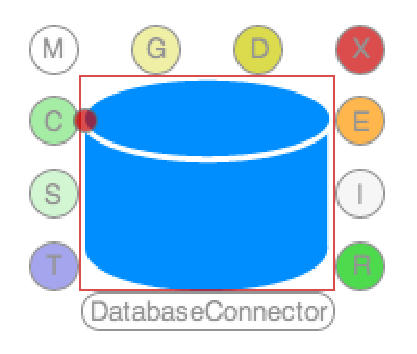
\includegraphics[width=0.3\textwidth]{figures/halos.pdf}
    \caption{The halo buttons of a simple morph.}
    \label{fig:Halos}
\end{figure}

Programmers can change the position of morphs by dragging and the composition by an alternative dragging, which is called \emph{grabbing}.
That is, the composition of morphs is also part of Morphic and a morph can have submorphs.
This way, morphs are not limited to to be basic shapes or simple widgets, but can be entire user interfaces of arbitrary applications.
Lively provides a set of manipulation tools, called \emph{Halos}, as shown in Figure~\ref{fig:Halos}, that developers can bring up directly at morphs.
The different halo buttons allow, for example, to resize~\textcircled{R}, rotate~\textcircled{T}, and copy~\textcircled{C} morphs.
The copy operation does not establish a prototypical inheritance relationship between the copy and the original, but instead copies the entire state, including of which class the copy is an instance.
Other halo buttons open specific tools, which are shown in Figure~\ref{fig:LivelyTools} to further manipulate the morphs:

\begin{enumerate}
    \item The \emph{Inspector}~\textcircled{1} presents all the values that make up a morph's state. It also has a small code pane at the bottom, which is intended to be used to manipulate the state programmatically.
    \item The \emph{Style Editor}~\textcircled{2} allows to manipulate certain aspects of a morph's visual appearance. Programmers can use it to, for example, change a morphs color, border width, or the layout of its submorphs.
    \item The \emph{Object Editor}~\textcircled{3} is a tool dedicated to the object-specific behavior of morphs, which are called \emph{scripts} in Lively. It shows all scripts of a particular morph, but also can add and adapt scripts.
\end{enumerate}

\begin{figure}[h]
    \centering
    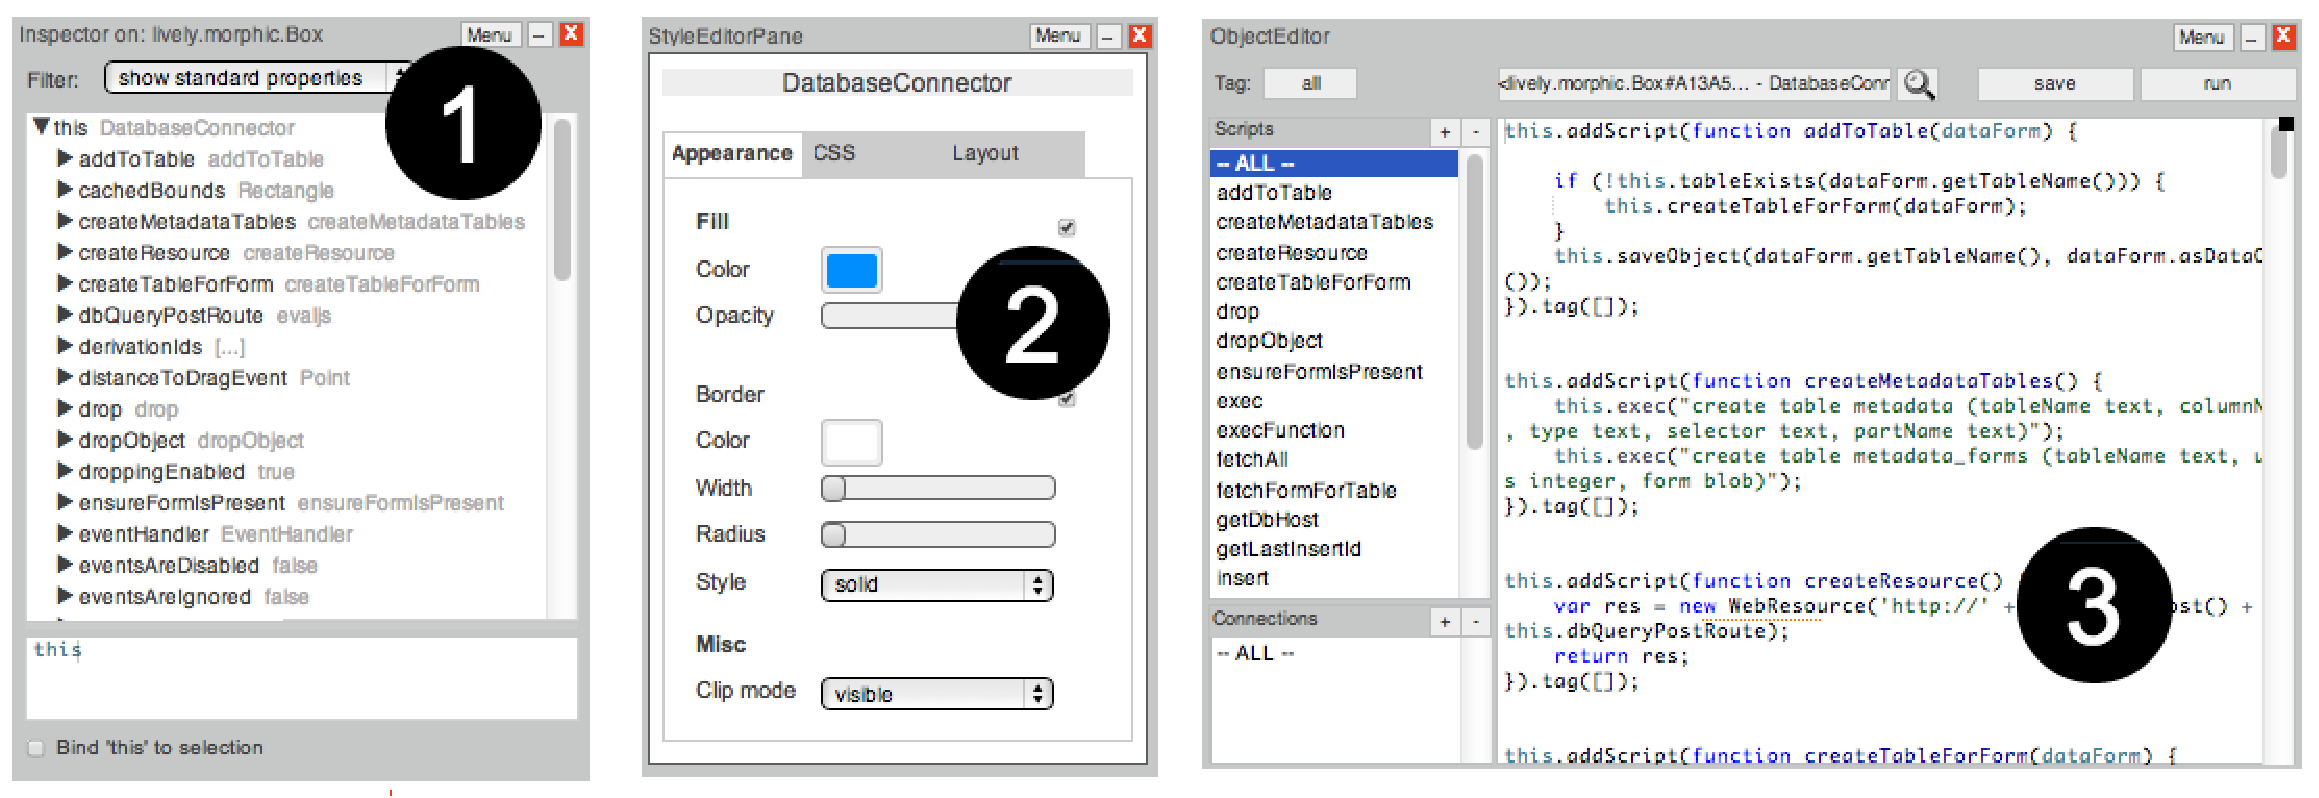
\includegraphics[width=\textwidth]{figures/livelyTools.pdf}
    \caption{Lively's tools to manipulate properties of morphs, from left to right: the Inspector, the Style Editor, and the Object Editor.}
    \label{fig:LivelyTools}
\end{figure}

\begin{figure}[h]
    \centering
    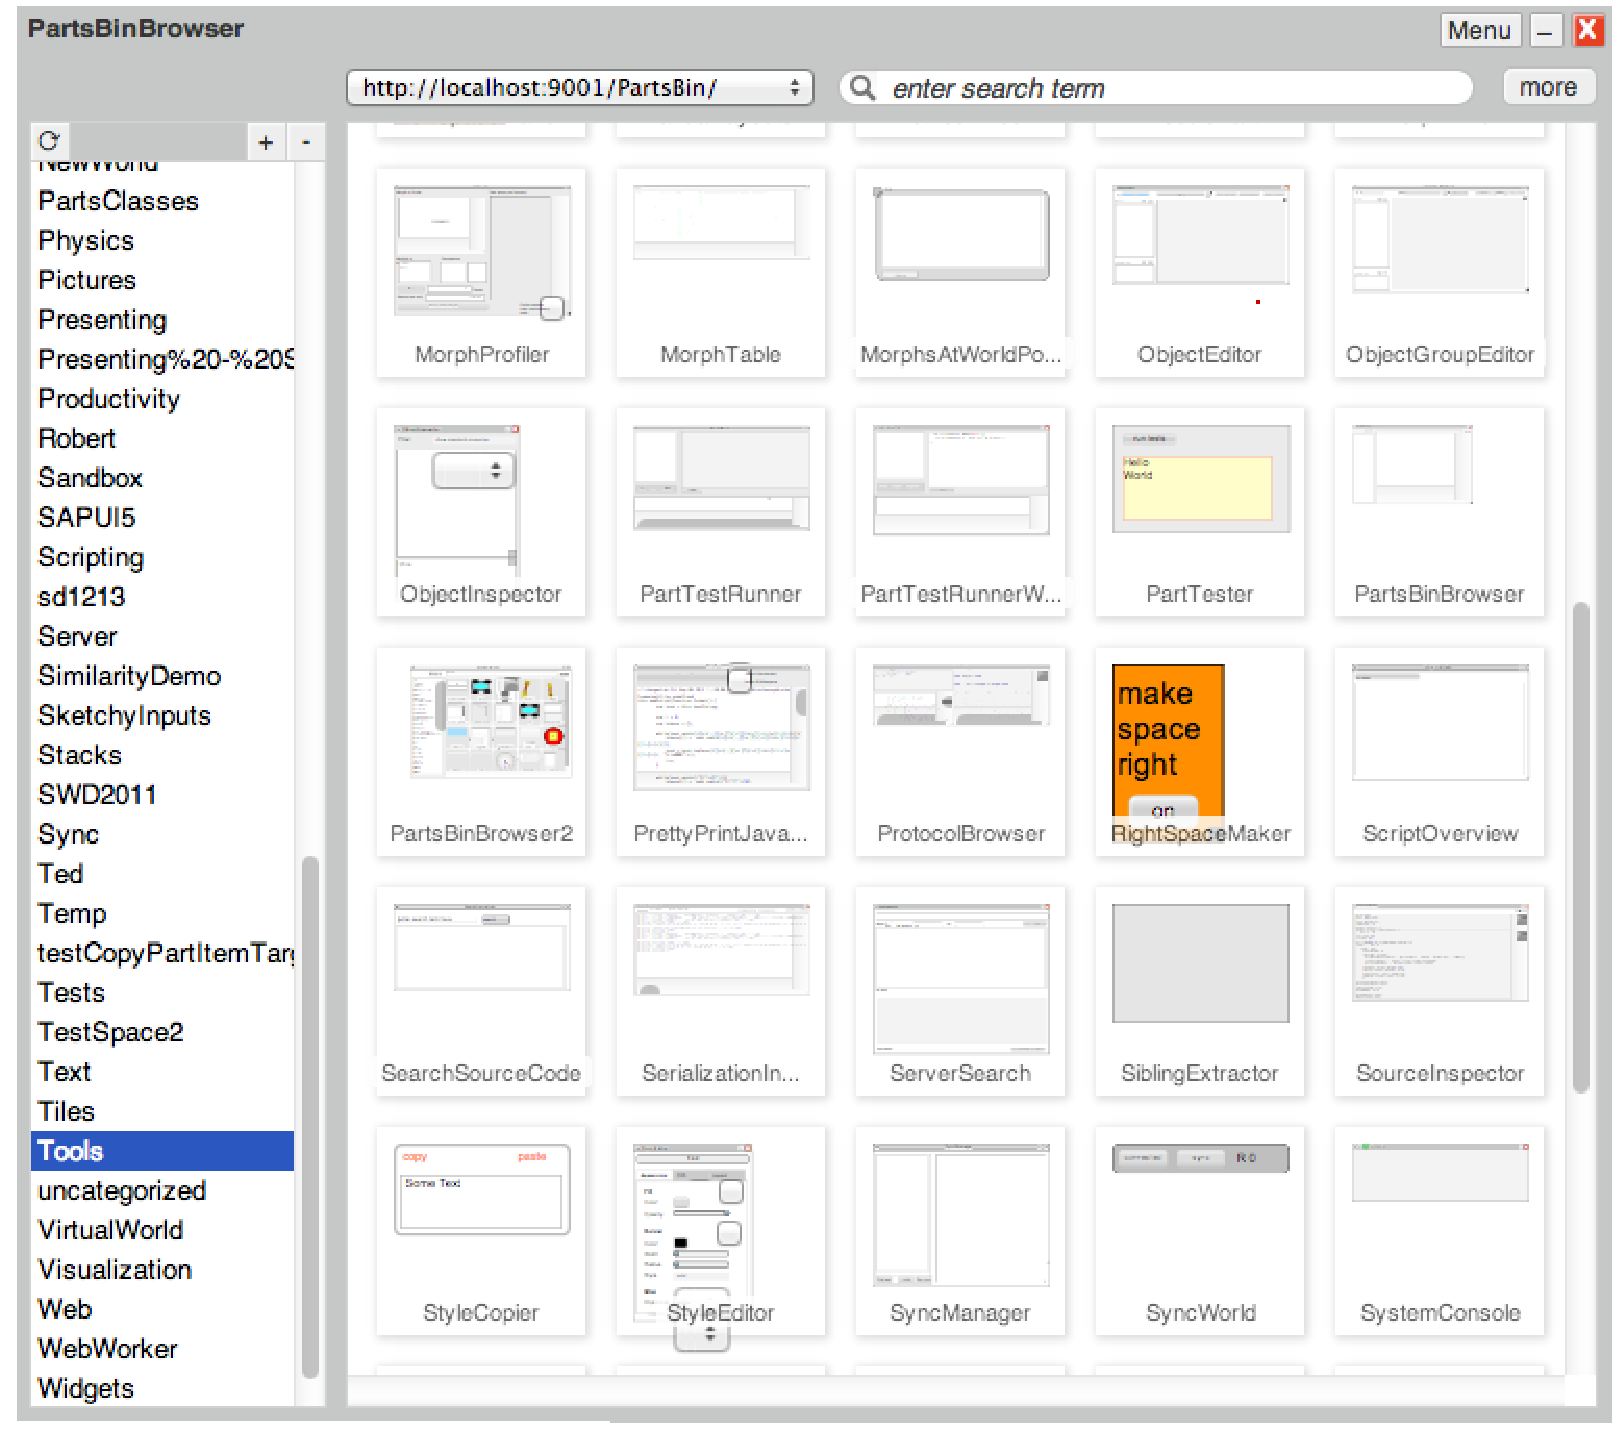
\includegraphics[width=0.7\textwidth]{figures/partsBin.pdf}
    \caption{Lively's Parts Bin opened on the \emph{Tools} category.}
    \label{fig:PartsBin}
\end{figure}

Another tool related to morphs, though not available from a halo button, is Lively's \emph{Parts Bin}~\cite{Lincke2012LPC}, an object repository to commit and load specific versions of morphs.
Morphs saved to the Parts Bin are called \emph{parts} to emphasize the ability to reuse any one of the morphic applications stored in the Parts Bin for other applications.
Figure~\ref{fig:PartsBin} shows the Parts Bin and, in particular, a group of tools that the Parts Bin contains, which includes both the Style Editor and the Object Editor.
Both these tools are examples for graphical applications developed from available parts, with their logic expressed in scripts, and available to users through the Parts Bin.


\section{CoExist}

The CoExist system\footnote{\url{http://www.bastiansteinert.org/coexist.html}, accessed February 28, 2014} and approach supports programmers through automatic and continuous versioning.
CoExist preserves each indermediate development state with its respective source code and associated runtime information.
The states are recorded as separate version in their original order and along with change summaries, associated test results, and screenshots of the development environment.
Programmers can review their development sessions, inspect the impact each individual change had on test cases, and recover previous development states.
They can completely withdraw withdraw changes or only re-visit a previous state to recover partial information as, for example, the source code for a specific method.

\begin{figure}[h]
    \centering
    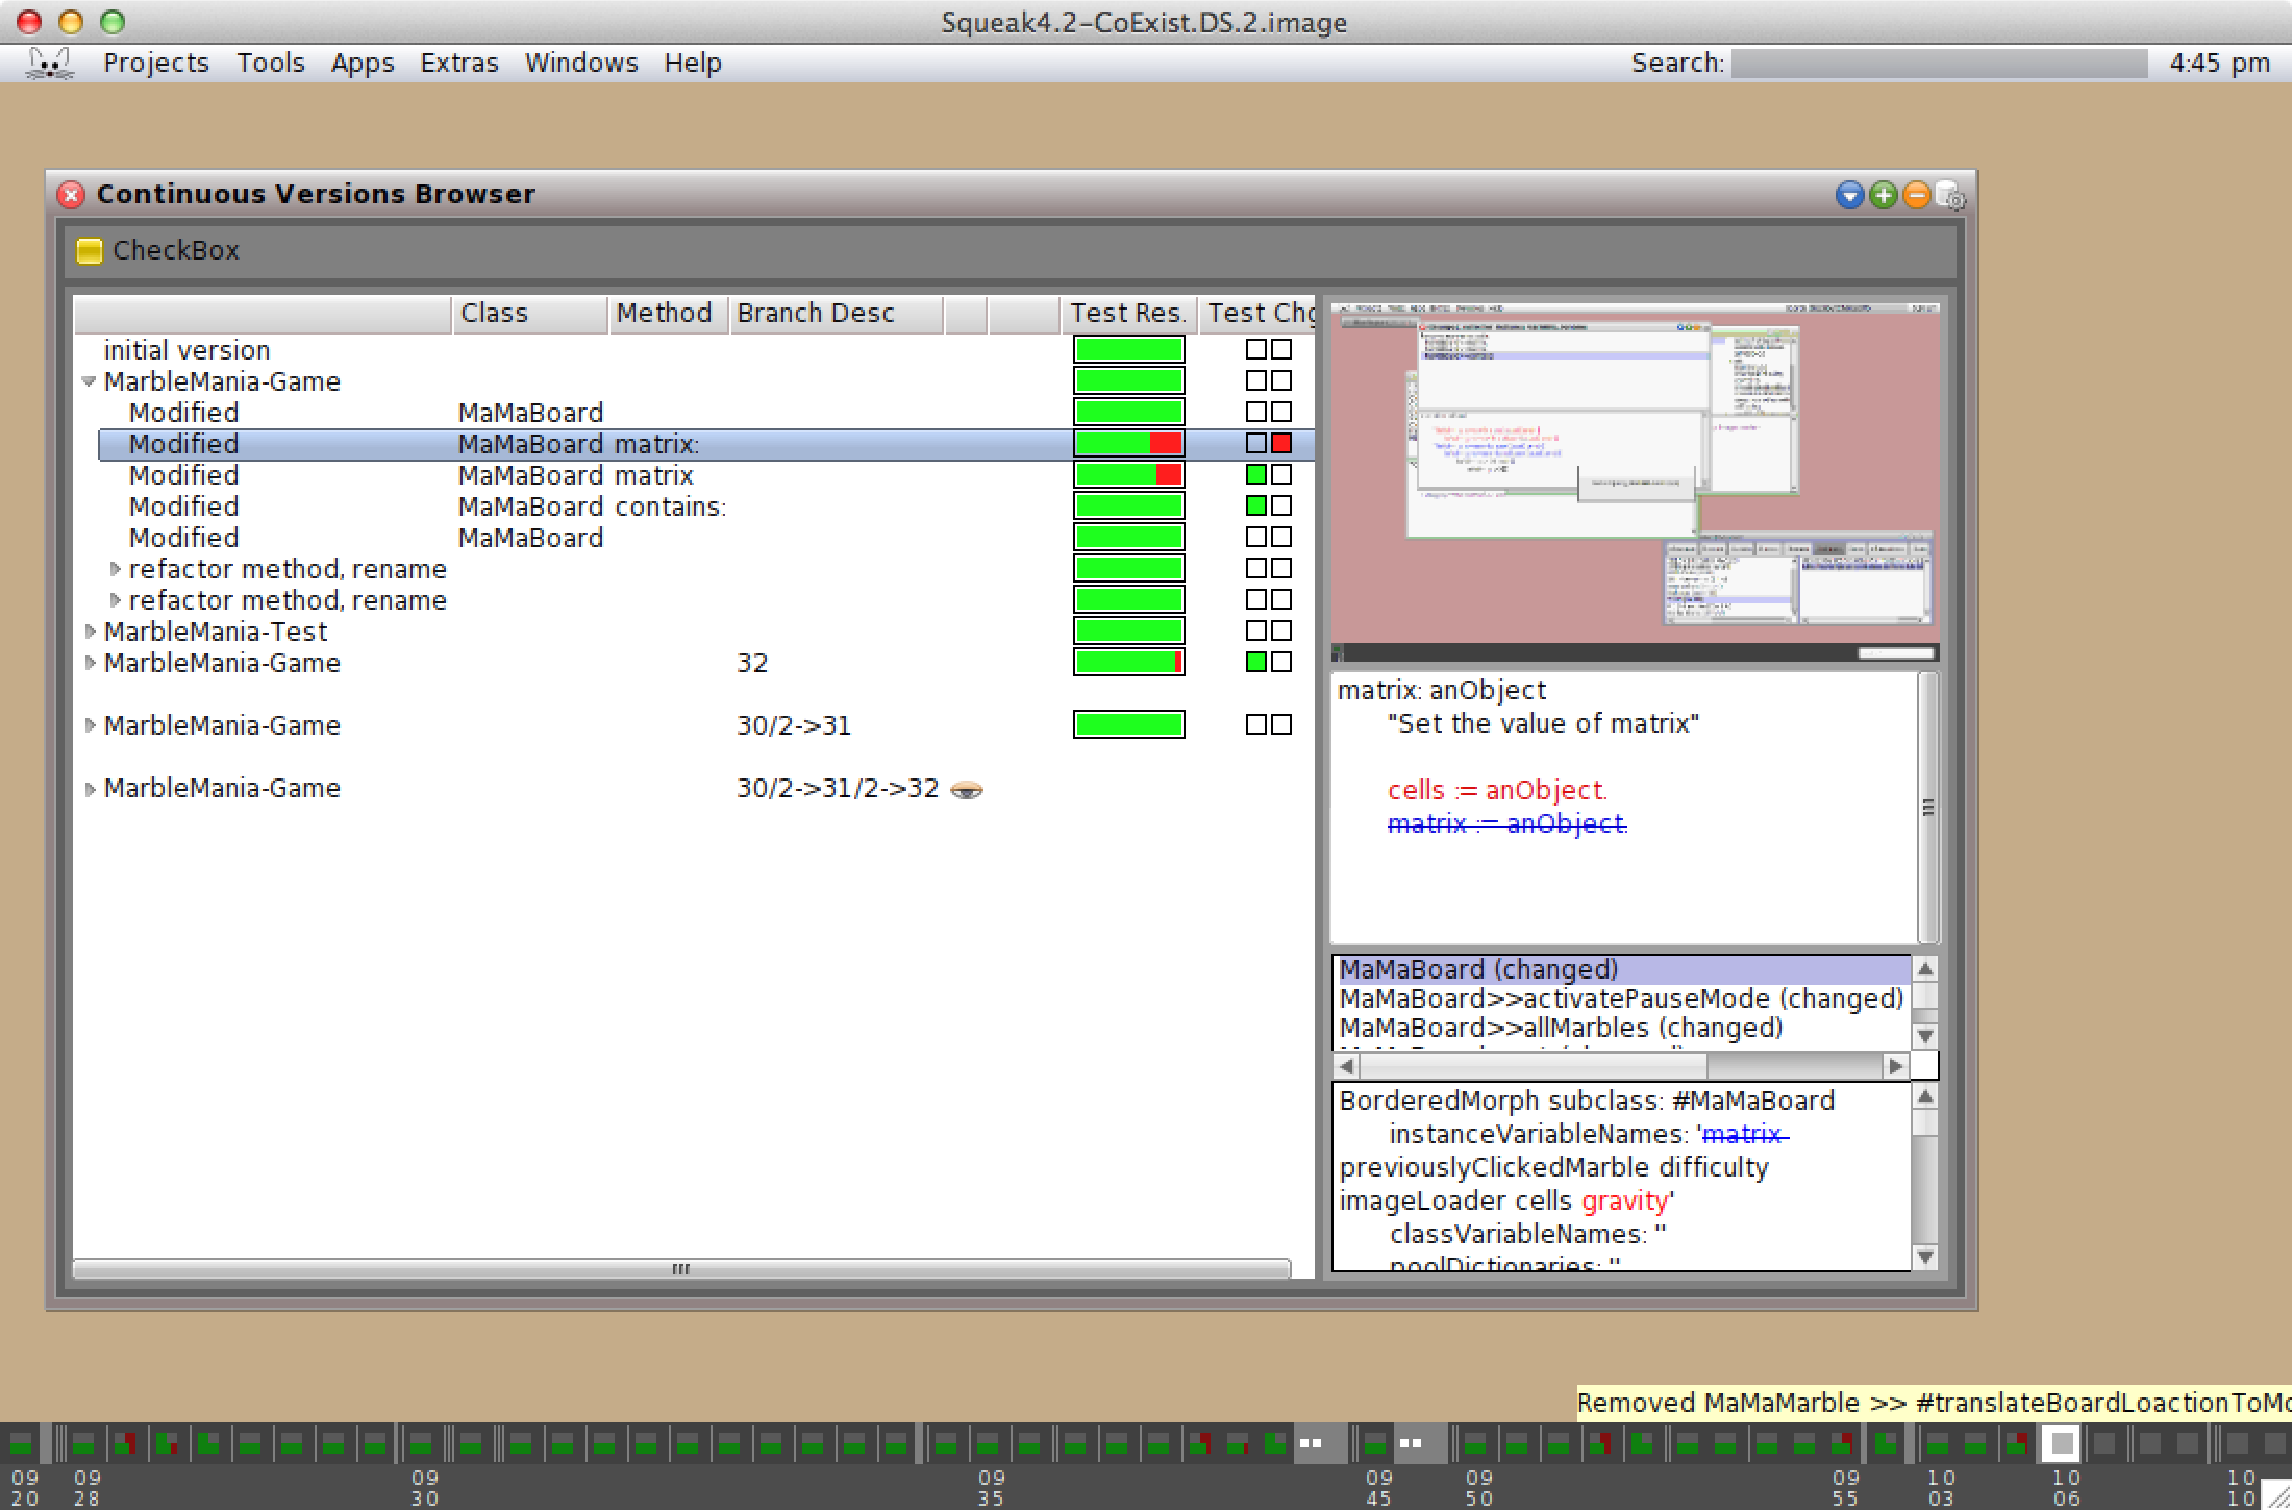
\includegraphics[width=\textwidth]{figures/coexistTools.pdf}
    \caption{CoExist's tools to manage the preserved development states: a timeline and a Version Browser.}
    \label{fig:CoExist}
\end{figure}

CoExist provides tools to help programmers benefit from the preserved development histories, shown in Figure~\ref{fig:CoExist}.
A timeline tool at the bottom of the development environment presents each intermediate version through a small rectangle that indicates the impact on test cases: the bottom of the rectangle shows how many test cases passed and failed absolutely, while the top half highlights only test results affected by the changes of this particular version.
Hovering above such a version rectangle indicates what exactly changed in terms of methods and classes.
Clicking a version provides access to its source code and more information on test results, but also allows to re-establish the version.
Besides this timeline of versions, a Version Browser tool shows changes in a different structure, also chronological, but separately for different source code modules.
It presents the same information on test cases, but in addition also offers diffs and how the development environment appeared visually in each version through providing screenshots.
The two tools support programmers in re-tracing their steps, understanding the impact of their actions, and in recovering information from previous development states.

CoExist is intented to reduce the effort that programmers usually put into recovery, either into actual compensational actions or into precautionary actions, and, thereby, also to help programmers to overcome any aversions to try new ideas.
To re-establish a previous development state---because of, for example, unintentionally introduced errors, decreased performance, or harmed program design---programmers can manually repair improperly changed code or load a previously commited version of the sources.
Programmers can preserve specific versions to be able to easily withdraw changes, and, thereby, reduce the cost of recovery by anticipating recovery needs beforehand.
However, preserving versions manually is also an effort and especially so when revision histories are expected to be well-documented and immediately useful.
For that, programmers need to assemble changes to meaningful increments, test these, and write helpful commit messages.
Testing each one directly is also advocated as it can help to find introduced problems directly intead of later analyzing long lists of changes that all could potentially have introduced a problem.
With CoExist, developers do not have to take these explicit precautionary actions, but still have access to a fine-grained history of development states and even test results for each individual state.
Instead of worrying about negative consequences when trying ideas, programmers can focus on their actual programming tasks and rely on CoExist to help in case any action unexpectedly needs to be undone.

% \todo{Structured: not just like auto-save (google docs), but structured: associated with particular actions and the static structure of programs... class>>method (add/delete/modify).. and also cross-document}

% % sometimes easier to make the changes and experience the results than to anticipate the changes beforehand...)… 